\documentclass[11pt,]{article}
\usepackage{lmodern}
\usepackage{amssymb,amsmath}
\usepackage{ifxetex,ifluatex}
\usepackage{fixltx2e} % provides \textsubscript
\ifnum 0\ifxetex 1\fi\ifluatex 1\fi=0 % if pdftex
  \usepackage[T1]{fontenc}
  \usepackage[utf8]{inputenc}
\else % if luatex or xelatex
  \ifxetex
    \usepackage{mathspec}
  \else
    \usepackage{fontspec}
  \fi
  \defaultfontfeatures{Ligatures=TeX,Scale=MatchLowercase}
\fi
% use upquote if available, for straight quotes in verbatim environments
\IfFileExists{upquote.sty}{\usepackage{upquote}}{}
% use microtype if available
\IfFileExists{microtype.sty}{%
\usepackage{microtype}
\UseMicrotypeSet[protrusion]{basicmath} % disable protrusion for tt fonts
}{}
\usepackage[margin=.75in]{geometry}
\usepackage{hyperref}
\hypersetup{unicode=true,
            pdftitle={Problem Set \#4},
            pdfauthor={Anaya Hall \& Christian Miller},
            pdfborder={0 0 0},
            breaklinks=true}
\urlstyle{same}  % don't use monospace font for urls
\usepackage{color}
\usepackage{fancyvrb}
\newcommand{\VerbBar}{|}
\newcommand{\VERB}{\Verb[commandchars=\\\{\}]}
\DefineVerbatimEnvironment{Highlighting}{Verbatim}{commandchars=\\\{\}}
% Add ',fontsize=\small' for more characters per line
\usepackage{framed}
\definecolor{shadecolor}{RGB}{248,248,248}
\newenvironment{Shaded}{\begin{snugshade}}{\end{snugshade}}
\newcommand{\KeywordTok}[1]{\textcolor[rgb]{0.13,0.29,0.53}{\textbf{#1}}}
\newcommand{\DataTypeTok}[1]{\textcolor[rgb]{0.13,0.29,0.53}{#1}}
\newcommand{\DecValTok}[1]{\textcolor[rgb]{0.00,0.00,0.81}{#1}}
\newcommand{\BaseNTok}[1]{\textcolor[rgb]{0.00,0.00,0.81}{#1}}
\newcommand{\FloatTok}[1]{\textcolor[rgb]{0.00,0.00,0.81}{#1}}
\newcommand{\ConstantTok}[1]{\textcolor[rgb]{0.00,0.00,0.00}{#1}}
\newcommand{\CharTok}[1]{\textcolor[rgb]{0.31,0.60,0.02}{#1}}
\newcommand{\SpecialCharTok}[1]{\textcolor[rgb]{0.00,0.00,0.00}{#1}}
\newcommand{\StringTok}[1]{\textcolor[rgb]{0.31,0.60,0.02}{#1}}
\newcommand{\VerbatimStringTok}[1]{\textcolor[rgb]{0.31,0.60,0.02}{#1}}
\newcommand{\SpecialStringTok}[1]{\textcolor[rgb]{0.31,0.60,0.02}{#1}}
\newcommand{\ImportTok}[1]{#1}
\newcommand{\CommentTok}[1]{\textcolor[rgb]{0.56,0.35,0.01}{\textit{#1}}}
\newcommand{\DocumentationTok}[1]{\textcolor[rgb]{0.56,0.35,0.01}{\textbf{\textit{#1}}}}
\newcommand{\AnnotationTok}[1]{\textcolor[rgb]{0.56,0.35,0.01}{\textbf{\textit{#1}}}}
\newcommand{\CommentVarTok}[1]{\textcolor[rgb]{0.56,0.35,0.01}{\textbf{\textit{#1}}}}
\newcommand{\OtherTok}[1]{\textcolor[rgb]{0.56,0.35,0.01}{#1}}
\newcommand{\FunctionTok}[1]{\textcolor[rgb]{0.00,0.00,0.00}{#1}}
\newcommand{\VariableTok}[1]{\textcolor[rgb]{0.00,0.00,0.00}{#1}}
\newcommand{\ControlFlowTok}[1]{\textcolor[rgb]{0.13,0.29,0.53}{\textbf{#1}}}
\newcommand{\OperatorTok}[1]{\textcolor[rgb]{0.81,0.36,0.00}{\textbf{#1}}}
\newcommand{\BuiltInTok}[1]{#1}
\newcommand{\ExtensionTok}[1]{#1}
\newcommand{\PreprocessorTok}[1]{\textcolor[rgb]{0.56,0.35,0.01}{\textit{#1}}}
\newcommand{\AttributeTok}[1]{\textcolor[rgb]{0.77,0.63,0.00}{#1}}
\newcommand{\RegionMarkerTok}[1]{#1}
\newcommand{\InformationTok}[1]{\textcolor[rgb]{0.56,0.35,0.01}{\textbf{\textit{#1}}}}
\newcommand{\WarningTok}[1]{\textcolor[rgb]{0.56,0.35,0.01}{\textbf{\textit{#1}}}}
\newcommand{\AlertTok}[1]{\textcolor[rgb]{0.94,0.16,0.16}{#1}}
\newcommand{\ErrorTok}[1]{\textcolor[rgb]{0.64,0.00,0.00}{\textbf{#1}}}
\newcommand{\NormalTok}[1]{#1}
\usepackage{longtable,booktabs}
\usepackage{graphicx,grffile}
\makeatletter
\def\maxwidth{\ifdim\Gin@nat@width>\linewidth\linewidth\else\Gin@nat@width\fi}
\def\maxheight{\ifdim\Gin@nat@height>\textheight\textheight\else\Gin@nat@height\fi}
\makeatother
% Scale images if necessary, so that they will not overflow the page
% margins by default, and it is still possible to overwrite the defaults
% using explicit options in \includegraphics[width, height, ...]{}
\setkeys{Gin}{width=\maxwidth,height=\maxheight,keepaspectratio}
\IfFileExists{parskip.sty}{%
\usepackage{parskip}
}{% else
\setlength{\parindent}{0pt}
\setlength{\parskip}{6pt plus 2pt minus 1pt}
}
\setlength{\emergencystretch}{3em}  % prevent overfull lines
\providecommand{\tightlist}{%
  \setlength{\itemsep}{0pt}\setlength{\parskip}{0pt}}
\setcounter{secnumdepth}{0}
% Redefines (sub)paragraphs to behave more like sections
\ifx\paragraph\undefined\else
\let\oldparagraph\paragraph
\renewcommand{\paragraph}[1]{\oldparagraph{#1}\mbox{}}
\fi
\ifx\subparagraph\undefined\else
\let\oldsubparagraph\subparagraph
\renewcommand{\subparagraph}[1]{\oldsubparagraph{#1}\mbox{}}
\fi

%%% Use protect on footnotes to avoid problems with footnotes in titles
\let\rmarkdownfootnote\footnote%
\def\footnote{\protect\rmarkdownfootnote}

%%% Change title format to be more compact
\usepackage{titling}

% Create subtitle command for use in maketitle
\newcommand{\subtitle}[1]{
  \posttitle{
    \begin{center}\large#1\end{center}
    }
}

\setlength{\droptitle}{-2em}
  \title{Problem Set \#4}
  \pretitle{\vspace{\droptitle}\centering\huge}
  \posttitle{\par}
  \author{Anaya Hall \& Christian Miller}
  \preauthor{\centering\large\emph}
  \postauthor{\par}
  \predate{\centering\large\emph}
  \postdate{\par}
  \date{Due April 25th}

\usepackage{booktabs}
\usepackage{longtable}
\usepackage{array}
\usepackage{multirow}
\usepackage[table]{xcolor}
\usepackage{wrapfig}
\usepackage{float}
\usepackage{colortbl}
\usepackage{pdflscape}
\usepackage{tabu}
\usepackage{threeparttable}
\usepackage[normalem]{ulem}

\begin{document}
\maketitle

\section{Serial Correlation}\label{serial-correlation}

The goal of this problem set is to explore what happens when we have
\emph{serially correlated distrubances}.

\subsection{Question 1}\label{question-1}

\textbf{Read the data into R. Plot the series against time and make sure
your data are read in correctly.} Also, print out data as ascii file and
compare the first and last row to make sure there's no funny business
with how the data were read in. Check a few points in the middle too.

\begin{Shaded}
\begin{Highlighting}[]
\CommentTok{# Column names from codebook}
\NormalTok{names <-}\StringTok{ }\KeywordTok{c}\NormalTok{(}\StringTok{"Year"}\NormalTok{, }\StringTok{"Qtr"}\NormalTok{, }\StringTok{"Realgdp"}\NormalTok{, }\StringTok{"Realcons"}\NormalTok{, }\StringTok{"Realinvs"}\NormalTok{, }\StringTok{"Realgovt"}\NormalTok{, }\StringTok{"Realdpi"}\NormalTok{, }\StringTok{"CPI_U"}\NormalTok{, }\StringTok{"M1"}\NormalTok{, }\StringTok{"Tbilrate"}\NormalTok{, }\StringTok{"Unemp"}\NormalTok{, }\StringTok{"Pop"}\NormalTok{, }\StringTok{"Infl"}\NormalTok{, }\StringTok{"Realint"}\NormalTok{)}

\CommentTok{# Read in txt file as data.frame using column names from codebook}
\NormalTok{gdp_data <-}\StringTok{ }\NormalTok{readr}\OperatorTok{::}\KeywordTok{read_table2}\NormalTok{(}\StringTok{"data.txt"}\NormalTok{,}
                             \DataTypeTok{col_names =}\NormalTok{ names) }
\end{Highlighting}
\end{Shaded}

\begin{Shaded}
\begin{Highlighting}[]
\CommentTok{#Plot the variables in our model against time}
\KeywordTok{ggplot}\NormalTok{(}\DataTypeTok{data =} \KeywordTok{gather}\NormalTok{(gdp_data, key, value, }\OperatorTok{-}\NormalTok{Year), }\KeywordTok{aes}\NormalTok{(}\DataTypeTok{x =}\NormalTok{ Year, }\DataTypeTok{y =}\NormalTok{ value)) }\OperatorTok{+}
\StringTok{  }\KeywordTok{geom_line}\NormalTok{() }\OperatorTok{+}
\StringTok{  }\KeywordTok{facet_wrap}\NormalTok{(}\OperatorTok{~}\StringTok{ }\NormalTok{key, }\DataTypeTok{scales =} \StringTok{"free"}\NormalTok{) }\OperatorTok{+}
\StringTok{  }\KeywordTok{ggtitle}\NormalTok{(}\StringTok{"GDP data variables over time"}\NormalTok{) }\OperatorTok{+}
\StringTok{  }\KeywordTok{ylab}\NormalTok{(}\StringTok{"Value"}\NormalTok{) }\OperatorTok{+}
\StringTok{  }\KeywordTok{xlab}\NormalTok{(}\StringTok{"Year"}\NormalTok{) }\OperatorTok{+}\StringTok{ }\KeywordTok{theme_minimal}\NormalTok{()}
\end{Highlighting}
\end{Shaded}

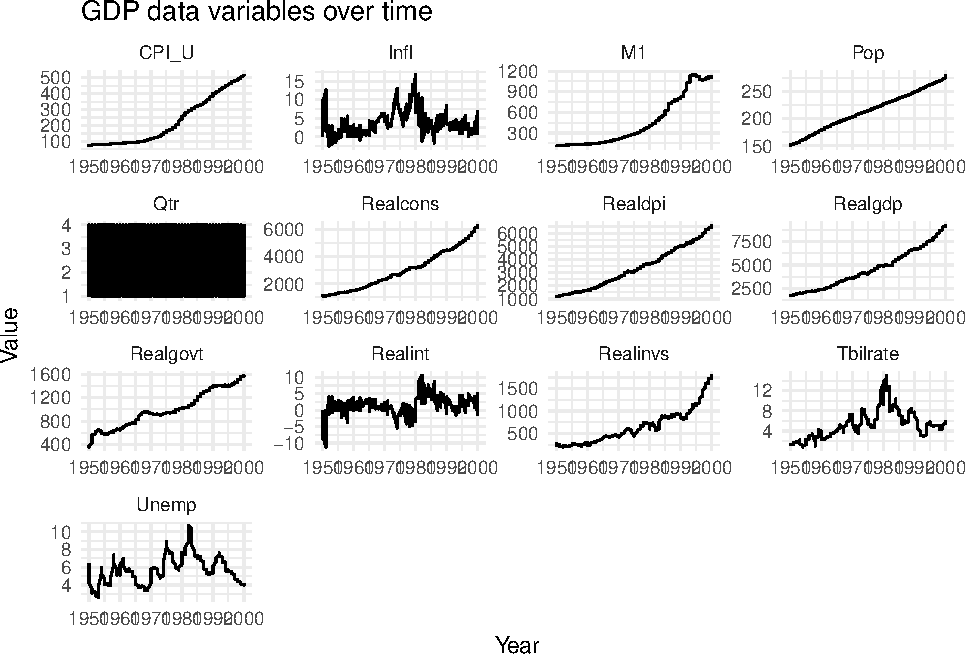
\includegraphics{ps4_code_files/figure-latex/plot_series-1.pdf}

\begin{Shaded}
\begin{Highlighting}[]
\KeywordTok{write.table}\NormalTok{(}\DataTypeTok{x =}\NormalTok{ gdp_data, }\DataTypeTok{file =} \StringTok{"test_ascii"}\NormalTok{)}

\CommentTok{# ascii(x = gdp_data, include.rownames = T)}
\end{Highlighting}
\end{Shaded}

So far, everthing looks good.

\subsection{Question 2: Phillips Curve}\label{question-2-phillips-curve}

Estimate the estimations augmented Phillips Curve (see Greene p.~251)

Equation:

\(\Delta p_t - \Delta p_{t-1} = \beta_1 + \beta_2\cdot u_t + \epsilon_t\)

\subsubsection{(a) Generate dependent
variable}\label{a-generate-dependent-variable}

\emph{Hint: Check the codebook; may need to drop one of our variables.}

Need to drop the first row because the first observation for Infl is
missing Phillip's curve regresses inflation (\%) on unemployment (\%)

\begin{Shaded}
\begin{Highlighting}[]
\CommentTok{# Generate Dependent Variable}
\ControlFlowTok{for}\NormalTok{ (i }\ControlFlowTok{in} \DecValTok{1}\OperatorTok{:}\KeywordTok{nrow}\NormalTok{(gdp_data)) \{}
                       \ControlFlowTok{if}\NormalTok{ (i}\OperatorTok{==}\DecValTok{1}\NormalTok{)}
\NormalTok{                       gdp_data}\OperatorTok{$}\NormalTok{delta_p[i] =}\StringTok{ }\OtherTok{NA}
                       \ControlFlowTok{else}
\NormalTok{                         gdp_data}\OperatorTok{$}\NormalTok{delta_p[i] =}\StringTok{ }\NormalTok{gdp_data}\OperatorTok{$}\NormalTok{Infl[i] }\OperatorTok{-}\StringTok{ }\NormalTok{gdp_data}\OperatorTok{$}\NormalTok{Infl[i}\OperatorTok{-}\DecValTok{1}\NormalTok{] \}}
\end{Highlighting}
\end{Shaded}

\begin{verbatim}
## Warning: Unknown or uninitialised column: 'delta_p'.
\end{verbatim}

\begin{Shaded}
\begin{Highlighting}[]
\CommentTok{# Drop first observation (row)}
\NormalTok{gdp_data <-}\StringTok{ }\NormalTok{gdp_data[}\OperatorTok{-}\DecValTok{1}\NormalTok{,]}
\end{Highlighting}
\end{Shaded}

\subsubsection{(b) Estimate relationship}\label{b-estimate-relationship}

Estimate relationship above. Report parameter estimates, standard
errors, t-statistics and \(R^2\).

First, let's load our OLS function.

\begin{Shaded}
\begin{Highlighting}[]
\CommentTok{# Function to convert tibble, data.frame, or tbl_df to matrix}
\NormalTok{to_matrix <-}\StringTok{ }\ControlFlowTok{function}\NormalTok{(the_df, vars) \{}
  \CommentTok{# Create a matrix from variables in var}
\NormalTok{  new_mat <-}\StringTok{ }\NormalTok{the_df }\OperatorTok
\StringTok{    }\CommentTok{#Select the columns given in 'vars'}
\StringTok{    }\KeywordTok{select_}\NormalTok{(}\DataTypeTok{.dots =}\NormalTok{ vars) }\OperatorTok
\StringTok{    }\CommentTok{# Convert to matrix}
\StringTok{    }\KeywordTok{as.matrix}\NormalTok{()}
  \CommentTok{# Return 'new_mat'}
  \KeywordTok{return}\NormalTok{(new_mat)}
\NormalTok{\}}


\NormalTok{b_ols <-}\StringTok{ }\ControlFlowTok{function}\NormalTok{(y, X) \{}
  \CommentTok{# Calculate beta hat}
\NormalTok{  beta_hat <-}\StringTok{ }\KeywordTok{solve}\NormalTok{(}\KeywordTok{t}\NormalTok{(X) }\OperatorTok\StringTok{ }\NormalTok{X) }\OperatorTok\StringTok{ }\KeywordTok{t}\NormalTok{(X) }\OperatorTok\StringTok{ }\NormalTok{y}
  \CommentTok{# Return beta_hat}
  \KeywordTok{return}\NormalTok{(beta_hat)}
\NormalTok{\}}

\NormalTok{ols <-}\StringTok{ }\ControlFlowTok{function}\NormalTok{(data, y_data, X_data, }\DataTypeTok{intercept =}\NormalTok{ T, }\DataTypeTok{H0 =} \DecValTok{0}\NormalTok{, }\DataTypeTok{two_tail =}\NormalTok{ T, }\DataTypeTok{alpha =} \FloatTok{0.05}\NormalTok{) \{}
  \CommentTok{# Function setup ----}
    \CommentTok{# Require the 'dplyr' package}
    \KeywordTok{require}\NormalTok{(dplyr)}
  
  \CommentTok{# Create dependent and independent variable matrices ----}
    \CommentTok{# y matrix}
\NormalTok{    y <-}\StringTok{ }\KeywordTok{to_matrix}\NormalTok{ (}\DataTypeTok{the_df =}\NormalTok{ data, }\DataTypeTok{vars =}\NormalTok{ y_data)}
    \CommentTok{# X matrix}
\NormalTok{    X <-}\StringTok{ }\KeywordTok{to_matrix}\NormalTok{ (}\DataTypeTok{the_df =}\NormalTok{ data, }\DataTypeTok{vars =}\NormalTok{ X_data)}
      \CommentTok{# If 'intercept' is TRUE, then add a column of ones}
      \ControlFlowTok{if}\NormalTok{ (intercept }\OperatorTok{==}\StringTok{ }\NormalTok{T) \{}
\NormalTok{      X <-}\StringTok{ }\KeywordTok{cbind}\NormalTok{(}\DecValTok{1}\NormalTok{,X)}
      \KeywordTok{colnames}\NormalTok{(X) <-}\StringTok{ }\KeywordTok{c}\NormalTok{(}\StringTok{"intercept"}\NormalTok{, X_data)}
\NormalTok{      \}}
 
  \CommentTok{# Calculate b, y_hat, and residuals ----}
\NormalTok{    b <-}\StringTok{ }\KeywordTok{solve}\NormalTok{(}\KeywordTok{t}\NormalTok{(X) }\OperatorTok\StringTok{ }\NormalTok{X) }\OperatorTok\StringTok{ }\KeywordTok{t}\NormalTok{(X) }\OperatorTok\StringTok{ }\NormalTok{y}
\NormalTok{    y_hat <-}\StringTok{ }\NormalTok{X }\OperatorTok\StringTok{ }\NormalTok{b}
\NormalTok{    e <-}\StringTok{ }\NormalTok{y }\OperatorTok{-}\StringTok{ }\NormalTok{y_hat}
    
  \CommentTok{# Useful -----}
\NormalTok{    n <-}\StringTok{ }\KeywordTok{nrow}\NormalTok{(X) }\CommentTok{# number of observations}
\NormalTok{    k <-}\StringTok{ }\KeywordTok{ncol}\NormalTok{(X) }\CommentTok{# number of independent variables}
\NormalTok{    dof <-}\StringTok{ }\NormalTok{n }\OperatorTok{-}\StringTok{ }\NormalTok{k }\CommentTok{# degrees of freedom}
\NormalTok{    i <-}\StringTok{ }\KeywordTok{rep}\NormalTok{(}\DecValTok{1}\NormalTok{,n) }\CommentTok{# column of ones for demeaning matrix}
\NormalTok{    A <-}\StringTok{ }\KeywordTok{diag}\NormalTok{(i) }\OperatorTok{-}\StringTok{ }\NormalTok{(}\DecValTok{1} \OperatorTok{/}\StringTok{ }\NormalTok{n) }\OperatorTok{*}\StringTok{ }\NormalTok{i }\OperatorTok\StringTok{ }\KeywordTok{t}\NormalTok{(i) }\CommentTok{# demeaning matrix}
\NormalTok{    y_star <-}\StringTok{ }\NormalTok{A }\OperatorTok\StringTok{ }\NormalTok{y }\CommentTok{# for SST}
\NormalTok{    X_star <-}\StringTok{ }\NormalTok{A }\OperatorTok\StringTok{ }\NormalTok{X }\CommentTok{# for SSM}
\NormalTok{    SST <-}\StringTok{ }\KeywordTok{drop}\NormalTok{(}\KeywordTok{t}\NormalTok{(y_star) }\OperatorTok\StringTok{ }\NormalTok{y_star)}
\NormalTok{    SSM <-}\StringTok{ }\KeywordTok{drop}\NormalTok{(}\KeywordTok{t}\NormalTok{(b) }\OperatorTok\StringTok{ }\KeywordTok{t}\NormalTok{(X_star) }\OperatorTok\StringTok{ }\NormalTok{X_star }\OperatorTok\StringTok{ }\NormalTok{b)}
\NormalTok{    SSR <-}\StringTok{ }\KeywordTok{drop}\NormalTok{(}\KeywordTok{t}\NormalTok{(e) }\OperatorTok\StringTok{ }\NormalTok{e)}
  
  \CommentTok{# Measures of fit and estimated variance ----}
\NormalTok{    R2uc <-}\StringTok{ }\KeywordTok{drop}\NormalTok{((}\KeywordTok{t}\NormalTok{(y_hat) }\OperatorTok\StringTok{ }\NormalTok{y_hat)}\OperatorTok{/}\NormalTok{(}\KeywordTok{t}\NormalTok{(y) }\OperatorTok\StringTok{ }\NormalTok{y)) }\CommentTok{# Uncentered R^2}
\NormalTok{    R2 <-}\StringTok{ }\DecValTok{1} \OperatorTok{-}\StringTok{ }\NormalTok{SSR}\OperatorTok{/}\NormalTok{SST }\CommentTok{# Uncentered R^2}
\NormalTok{    R2adj <-}\StringTok{ }\DecValTok{1} \OperatorTok{-}\StringTok{ }\NormalTok{(n}\OperatorTok{-}\DecValTok{1}\NormalTok{)}\OperatorTok{/}\NormalTok{dof }\OperatorTok{*}\StringTok{ }\NormalTok{(}\DecValTok{1} \OperatorTok{-}\StringTok{ }\NormalTok{R2) }\CommentTok{# Adjusted R^2}
\NormalTok{    AIC <-}\StringTok{ }\KeywordTok{log}\NormalTok{(SSR}\OperatorTok{/}\NormalTok{n) }\OperatorTok{+}\StringTok{ }\DecValTok{2}\OperatorTok{*}\NormalTok{k}\OperatorTok{/}\NormalTok{n }\CommentTok{# AIC}
\NormalTok{    SIC <-}\StringTok{ }\KeywordTok{log}\NormalTok{(SSR}\OperatorTok{/}\NormalTok{n) }\OperatorTok{+}\StringTok{ }\NormalTok{k}\OperatorTok{/}\NormalTok{n}\OperatorTok{*}\KeywordTok{log}\NormalTok{(n) }\CommentTok{# SIC}
\NormalTok{    s2 <-}\StringTok{ }\NormalTok{SSR}\OperatorTok{/}\NormalTok{dof }\CommentTok{# s^2}
  
  \CommentTok{# Measures of fit table ----}
\NormalTok{    mof_table_df <-}\StringTok{ }\KeywordTok{data.frame}\NormalTok{(R2uc, R2, R2adj, SIC, AIC, SSR, s2)}
\NormalTok{    mof_table_col_names <-}\StringTok{ }\KeywordTok{c}\NormalTok{(}\StringTok{"$R^2_}\CharTok{\textbackslash{}\textbackslash{}}\StringTok{text\{uc\}$"}\NormalTok{, }\StringTok{"$R^2$"}\NormalTok{,}
                             \StringTok{"$R^2_}\CharTok{\textbackslash{}\textbackslash{}}\StringTok{text\{adj\}$"}\NormalTok{,}
                             \StringTok{"SIC"}\NormalTok{, }\StringTok{"AIC"}\NormalTok{, }\StringTok{"SSR"}\NormalTok{, }\StringTok{"$s^2$"}\NormalTok{)}
\NormalTok{    mof_table <-}\StringTok{  }\NormalTok{mof_table_df }\OperatorTok\StringTok{ }\NormalTok{knitr}\OperatorTok{::}\KeywordTok{kable}\NormalTok{(}
      \DataTypeTok{row.names =}\NormalTok{ F,}
      \DataTypeTok{col.names =}\NormalTok{ mof_table_col_names,}
      \DataTypeTok{format.args =} \KeywordTok{list}\NormalTok{(}\DataTypeTok{scientific =}\NormalTok{ F, }\DataTypeTok{digits =} \DecValTok{4}\NormalTok{),}
      \DataTypeTok{booktabs =}\NormalTok{ T,}
      \DataTypeTok{escape =}\NormalTok{ F}
\NormalTok{    )}
  
  \CommentTok{# t-test----}
    \CommentTok{# Standard error}
\NormalTok{    se <-}\StringTok{ }\KeywordTok{as.vector}\NormalTok{(}\KeywordTok{sqrt}\NormalTok{(s2 }\OperatorTok{*}\StringTok{ }\KeywordTok{diag}\NormalTok{(}\KeywordTok{solve}\NormalTok{(}\KeywordTok{t}\NormalTok{(X) }\OperatorTok\StringTok{ }\NormalTok{X))))}
    \CommentTok{# Vector of _t_ statistics}
\NormalTok{    t_stats <-}\StringTok{ }\NormalTok{(b }\OperatorTok{-}\StringTok{ }\NormalTok{H0) }\OperatorTok{/}\StringTok{ }\NormalTok{se}
    \CommentTok{# Calculate the p-values}
    \ControlFlowTok{if}\NormalTok{ (two_tail }\OperatorTok{==}\StringTok{ }\NormalTok{T) \{}
\NormalTok{    p_values <-}\StringTok{ }\KeywordTok{pt}\NormalTok{(}\DataTypeTok{q =} \KeywordTok{abs}\NormalTok{(t_stats), }\DataTypeTok{df =}\NormalTok{ dof, }\DataTypeTok{lower.tail =}\NormalTok{ F) }\OperatorTok{*}\StringTok{ }\DecValTok{2}
\NormalTok{    \} }\ControlFlowTok{else}\NormalTok{ \{}
\NormalTok{      p_values <-}\StringTok{ }\KeywordTok{pt}\NormalTok{(}\DataTypeTok{q =} \KeywordTok{abs}\NormalTok{(t_stats), }\DataTypeTok{df =}\NormalTok{ dof, }\DataTypeTok{lower.tail =}\NormalTok{ F)}
\NormalTok{    \}}
    \CommentTok{# Do we (fail to) reject?}
\NormalTok{    reject <-}\StringTok{ }\KeywordTok{ifelse}\NormalTok{(p_values }\OperatorTok{<}\StringTok{ }\NormalTok{alpha, reject <-}\StringTok{ "Reject"}\NormalTok{, reject <-}\StringTok{ "Fail to Reject"}\NormalTok{)}
    
    \CommentTok{# Nice table (data.frame) of results}
\NormalTok{    ttest_df <-}\StringTok{ }\KeywordTok{data.frame}\NormalTok{(}
      \CommentTok{# The rows have the coef. names}
      \DataTypeTok{effect =} \KeywordTok{rownames}\NormalTok{(b),}
      \CommentTok{# Estimated coefficients}
      \DataTypeTok{coef =} \KeywordTok{as.vector}\NormalTok{(b) }\OperatorTok\StringTok{ }\KeywordTok{round}\NormalTok{(}\DecValTok{3}\NormalTok{),}
      \CommentTok{# Standard errors}
      \DataTypeTok{std_error =} \KeywordTok{as.vector}\NormalTok{(se) }\OperatorTok\StringTok{ }\KeywordTok{round}\NormalTok{(}\DecValTok{4}\NormalTok{),}
      \CommentTok{# t statistics}
      \DataTypeTok{t_stat =} \KeywordTok{as.vector}\NormalTok{(t_stats) }\OperatorTok\StringTok{ }\KeywordTok{round}\NormalTok{(}\DecValTok{3}\NormalTok{),}
      \CommentTok{# p-values}
      \DataTypeTok{p_value =} \KeywordTok{as.vector}\NormalTok{(p_values) }\OperatorTok\StringTok{ }\KeywordTok{round}\NormalTok{(}\DecValTok{4}\NormalTok{),}
      \CommentTok{# reject null?}
      \DataTypeTok{significance =} \KeywordTok{as.character}\NormalTok{(reject)}
\NormalTok{      )}
  
\NormalTok{    ttest_table <-}\StringTok{  }\NormalTok{ttest_df }\OperatorTok\StringTok{ }\NormalTok{knitr}\OperatorTok{::}\KeywordTok{kable}\NormalTok{(}
      \DataTypeTok{col.names =} \KeywordTok{c}\NormalTok{(}\StringTok{""}\NormalTok{, }\StringTok{"Coef."}\NormalTok{, }\StringTok{"S.E."}\NormalTok{, }\StringTok{"t Stat"}\NormalTok{, }\StringTok{"p-Value"}\NormalTok{, }\StringTok{"Decision"}\NormalTok{),}
      \DataTypeTok{booktabs =}\NormalTok{ T,}
      \DataTypeTok{format.args =} \KeywordTok{list}\NormalTok{(}\DataTypeTok{scientific =}\NormalTok{ F),}
      \DataTypeTok{escape =}\NormalTok{ F,}
      \DataTypeTok{caption =} \StringTok{"OLS Results"}
\NormalTok{    )}

  \CommentTok{# Data frame for exporting for y, y_hat, X, and e vectors ----}
\NormalTok{    export_df <-}\StringTok{ }\KeywordTok{data.frame}\NormalTok{(y, y_hat, e, X) }\OperatorTok\StringTok{ }\KeywordTok{tbl_df}\NormalTok{()}
    \KeywordTok{colnames}\NormalTok{(export_df) <-}\StringTok{ }\KeywordTok{c}\NormalTok{(}\StringTok{"y"}\NormalTok{,}\StringTok{"y_hat"}\NormalTok{,}\StringTok{"e"}\NormalTok{,}\KeywordTok{colnames}\NormalTok{(X))}
  
  \CommentTok{# Return ----}
    \KeywordTok{return}\NormalTok{(}\KeywordTok{list}\NormalTok{(}\DataTypeTok{n=}\NormalTok{n, }\DataTypeTok{dof=}\NormalTok{dof, }\DataTypeTok{b=}\NormalTok{b, }\DataTypeTok{vars=}\NormalTok{export_df, }\DataTypeTok{R2uc=}\NormalTok{R2uc,}\DataTypeTok{R2=}\NormalTok{R2,}
                \DataTypeTok{R2adj=}\NormalTok{R2adj, }\DataTypeTok{AIC=}\NormalTok{AIC, }\DataTypeTok{SIC=}\NormalTok{SIC, }\DataTypeTok{s2=}\NormalTok{s2, }\DataTypeTok{SST=}\NormalTok{SST, }\DataTypeTok{SSR=}\NormalTok{SSR,}
                \DataTypeTok{mof_table=}\NormalTok{mof_table, }\DataTypeTok{ttest=}\NormalTok{ttest_table))}
\NormalTok{\}}
\end{Highlighting}
\end{Shaded}

\newpage

\begin{Shaded}
\begin{Highlighting}[]
\CommentTok{# What is the right model here??--- all covariates?}
\NormalTok{## I dropped }
\NormalTok{covariates <-}\StringTok{ }\KeywordTok{c}\NormalTok{(}\StringTok{"Year"}\NormalTok{, }\StringTok{"Qtr"}\NormalTok{, }\StringTok{"Realgdp"}\NormalTok{, }\StringTok{"Realcons"}\NormalTok{, }\StringTok{"Realinvs"}\NormalTok{, }\StringTok{"Realgovt"}\NormalTok{, }\StringTok{"Realdpi"}\NormalTok{, }\StringTok{"CPI_U"}\NormalTok{, }\StringTok{"M1"}\NormalTok{, }\StringTok{"Tbilrate"}\NormalTok{, }\StringTok{"Unemp"}\NormalTok{, }\StringTok{"Pop"}\NormalTok{, }\StringTok{"Infl"}\NormalTok{, }\StringTok{"Realint"}\NormalTok{)}

\NormalTok{model_}\DecValTok{1}\NormalTok{ <-}\StringTok{ }\KeywordTok{ols}\NormalTok{(gdp_data, }
               \DataTypeTok{y_data =} \StringTok{"delta_p"}\NormalTok{, }
               \DataTypeTok{X_data =}\KeywordTok{c}\NormalTok{(}\StringTok{"Year"}\NormalTok{, }\StringTok{"Realgdp"}\NormalTok{, }\StringTok{"Realcons"}\NormalTok{, }\StringTok{"Realinvs"}\NormalTok{, }\StringTok{"Realgovt"}\NormalTok{, }\StringTok{"Realdpi"}\NormalTok{, }\StringTok{"CPI_U"}\NormalTok{, }\StringTok{"M1"}\NormalTok{, }\StringTok{"Tbilrate"}\NormalTok{, }\StringTok{"Unemp"}\NormalTok{, }\StringTok{"Pop"}\NormalTok{, }\StringTok{"Infl"}\NormalTok{, }\StringTok{"Realint"}\NormalTok{))}

\NormalTok{model_}\DecValTok{1}\OperatorTok{$}\NormalTok{ttest}
\end{Highlighting}
\end{Shaded}

\begin{longtable}[]{@{}lrrrrl@{}}
\caption{OLS Results}\tabularnewline
\toprule
& Coef. & S.E. & t Stat & p-Value & Decision\tabularnewline
\midrule
\endfirsthead
\toprule
& Coef. & S.E. & t Stat & p-Value & Decision\tabularnewline
\midrule
\endhead
intercept & -1932.304 & 811.8926 & -2.380 & 0.0183 &
Reject\tabularnewline
Year & 1.004 & 0.4265 & 2.353 & 0.0196 & Reject\tabularnewline
Realgdp & -0.023 & 0.0056 & -4.072 & 0.0001 & Reject\tabularnewline
Realcons & 0.018 & 0.0065 & 2.760 & 0.0064 & Reject\tabularnewline
Realinvs & 0.022 & 0.0053 & 4.189 & 0.0000 & Reject\tabularnewline
Realgovt & 0.020 & 0.0059 & 3.321 & 0.0011 & Reject\tabularnewline
Realdpi & -0.006 & 0.0041 & -1.491 & 0.1376 & Fail to
Reject\tabularnewline
CPI\_U & 0.040 & 0.0172 & 2.301 & 0.0225 & Reject\tabularnewline
M1 & 0.002 & 0.0054 & 0.456 & 0.6488 & Fail to Reject\tabularnewline
Tbilrate & 84.176 & 62.7045 & 1.342 & 0.1811 & Fail to
Reject\tabularnewline
Unemp & -0.328 & 0.3383 & -0.970 & 0.3333 & Fail to
Reject\tabularnewline
Pop & -0.103 & 0.1444 & -0.716 & 0.4751 & Fail to Reject\tabularnewline
Infl & -83.903 & 62.6919 & -1.338 & 0.1824 & Fail to
Reject\tabularnewline
Realint & -84.650 & 62.7006 & -1.350 & 0.1786 & Fail to
Reject\tabularnewline
\bottomrule
\end{longtable}

\begin{Shaded}
\begin{Highlighting}[]
\NormalTok{model_}\DecValTok{1}\OperatorTok{$}\NormalTok{mof_table}
\end{Highlighting}
\end{Shaded}

\begin{longtable}[]{@{}rrrrrrr@{}}
\toprule
\(R^2_\text{uc}\) & \(R^2\) & \(R^2_\text{adj}\) & SIC & AIC & SSR &
\(s^2\)\tabularnewline
\midrule
\endhead
0.386 & 0.386 & 0.3438 & 1.954 & 1.725 & 992.7 & 5.252\tabularnewline
\bottomrule
\end{longtable}

\subsubsection{(c) Plot residuals against
time}\label{c-plot-residuals-against-time}

\begin{Shaded}
\begin{Highlighting}[]
\NormalTok{res <-}\StringTok{ }\NormalTok{model_}\DecValTok{1}\OperatorTok{$}\NormalTok{vars}\OperatorTok{$}\NormalTok{e}

\KeywordTok{plot}\NormalTok{(gdp_data}\OperatorTok{$}\NormalTok{Year, res)}
\end{Highlighting}
\end{Shaded}

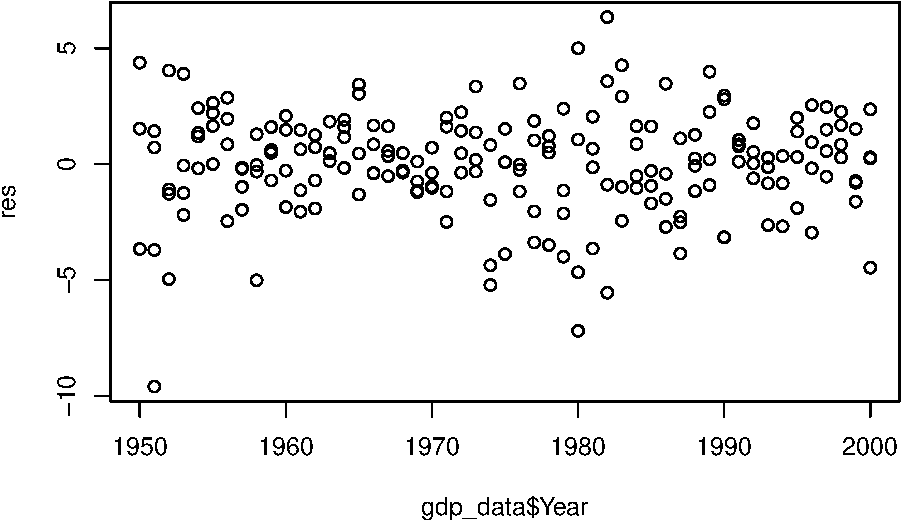
\includegraphics{ps4_code_files/figure-latex/plot_resid-1.pdf} Looking
at this plot, we likely have a POSITVE auto-correlation issue\ldots{}.

\subsubsection{(d) Breusch-Godfrey}\label{d-breusch-godfrey}

Use Breusch-Godfrey test to test for first order correlation

Procedure 1. Run OLS \& save residuals 2. Augment with column of lagged
residuals --\textgreater{} X0 (fill in any NAs with zeros) 3. Auxillary
regression: regress residuals et on X0t 4. Test Statistic:

\(LM = T \cdot R^2_0\)

Null hypothesis is no serial correlation

\begin{Shaded}
\begin{Highlighting}[]
\CommentTok{# BGX_data <- select(gdp_data, c("Year", "Realgdp", "Realcons", "Realinvs", "Realgovt", "Realdpi", "CPI_U", "M1", "Tbilrate", "Unemp", "Pop", "Infl", "Realint"))}

\CommentTok{# First order only}
\NormalTok{BGtest <-}\StringTok{ }\ControlFlowTok{function}\NormalTok{(data, y_data, X_data, }\DataTypeTok{order =} \DecValTok{1}\NormalTok{) \{}
\NormalTok{  y <-}\StringTok{ }\KeywordTok{to_matrix}\NormalTok{(data, y_data)}
\NormalTok{  X <-}\StringTok{ }\KeywordTok{to_matrix}\NormalTok{(data, X_data)}
\NormalTok{  Z <-}\StringTok{ }\KeywordTok{to_matrix}\NormalTok{(data, X_data)}
  
  \CommentTok{# Run OLS and save residuals to new covariate matrix}
\NormalTok{  e0 <-}\StringTok{ }\KeywordTok{ols}\NormalTok{(data, y_data, X_data)}\OperatorTok{$}\NormalTok{vars}\OperatorTok{$}\NormalTok{e}
\NormalTok{  Z <-}\StringTok{ }\KeywordTok{cbind}\NormalTok{(Z, e0)}
  
  \CommentTok{# Add column of for lagged residuals}
\NormalTok{  Z <-}\StringTok{ }\KeywordTok{cbind}\NormalTok{(}\OtherTok{NA}\NormalTok{, Z)}
  \KeywordTok{colnames}\NormalTok{(Z)[}\DecValTok{1}\NormalTok{] <-}\StringTok{ "e_lag"}

  \CommentTok{# First, convert Z to dataframe for lagging operation}
\NormalTok{  c <-}\StringTok{ }\KeywordTok{as.data.frame}\NormalTok{(Z)}
  
  \CommentTok{# Create lagged residuals}
    \ControlFlowTok{for}\NormalTok{ (i }\ControlFlowTok{in} \DecValTok{1}\OperatorTok{:}\KeywordTok{nrow}\NormalTok{(Z)) \{}
    \ControlFlowTok{if}\NormalTok{ (i }\OperatorTok{==}\StringTok{ }\DecValTok{1}\NormalTok{)}
\NormalTok{      c}\OperatorTok{$}\NormalTok{e_lag[[i]] =}\StringTok{ }\DecValTok{0}
    \ControlFlowTok{else}
\NormalTok{      c}\OperatorTok{$}\NormalTok{e_lag[[i]] =}\StringTok{ }\NormalTok{c}\OperatorTok{$}\NormalTok{e0[i}\OperatorTok{-}\DecValTok{1}\NormalTok{]}
\NormalTok{    \}}

  \CommentTok{# Back to matrix}
\NormalTok{  X0 <-}\StringTok{ }\NormalTok{c[}\OperatorTok{-}\KeywordTok{ncol}\NormalTok{(c)] }\OperatorTok\StringTok{ }\KeywordTok{as.matrix}\NormalTok{()}
  \CommentTok{# BG_df <- cbind(data[y_data], X0)}
\NormalTok{  BG_df <-}\StringTok{ }\NormalTok{c}

  \CommentTok{# Regress}
\NormalTok{  R2_stat <-}\StringTok{ }\KeywordTok{ols}\NormalTok{(BG_df, }\StringTok{"e0"}\NormalTok{, }\KeywordTok{colnames}\NormalTok{(X0))}\OperatorTok{$}\NormalTok{R2}
\NormalTok{  test_stat <-}\StringTok{ }\NormalTok{R2_stat}\OperatorTok{*}\KeywordTok{nrow}\NormalTok{(data)}
  
\NormalTok{  pvalue <-}\StringTok{ }\DecValTok{1} \OperatorTok{-}\StringTok{ }\KeywordTok{pchisq}\NormalTok{(test_stat, }\DataTypeTok{df =} \DecValTok{1}\NormalTok{)}
    
  \KeywordTok{return}\NormalTok{(}\KeywordTok{data_frame}\NormalTok{(}\StringTok{"Test Statistic"}\NormalTok{ =}\StringTok{ }\NormalTok{test_stat, }
              \StringTok{"P-Value"}\NormalTok{ =}\StringTok{ }\NormalTok{pvalue))}
  
\NormalTok{\}}

\KeywordTok{BGtest}\NormalTok{(}\DataTypeTok{data =}\NormalTok{ gdp_data, }\DataTypeTok{y_data =} \StringTok{"delta_p"}\NormalTok{, }\DataTypeTok{X_data =} \KeywordTok{c}\NormalTok{(}\StringTok{"Year"}\NormalTok{, }\StringTok{"Realgdp"}\NormalTok{, }\StringTok{"Realcons"}\NormalTok{, }\StringTok{"Realinvs"}\NormalTok{, }\StringTok{"Realgovt"}\NormalTok{, }\StringTok{"Realdpi"}\NormalTok{, }\StringTok{"CPI_U"}\NormalTok{, }\StringTok{"M1"}\NormalTok{, }\StringTok{"Tbilrate"}\NormalTok{, }\StringTok{"Unemp"}\NormalTok{, }\StringTok{"Pop"}\NormalTok{, }\StringTok{"Infl"}\NormalTok{, }\StringTok{"Realint"}\NormalTok{)) }\OperatorTok\StringTok{ }\NormalTok{knitr}\OperatorTok{::}\KeywordTok{kable}\NormalTok{()}
\end{Highlighting}
\end{Shaded}

\begin{longtable}[]{@{}rr@{}}
\toprule
Test Statistic & P-Value\tabularnewline
\midrule
\endhead
0.3518258 & 0.5530814\tabularnewline
\bottomrule
\end{longtable}

\begin{Shaded}
\begin{Highlighting}[]
\CommentTok{# ols(data = gdp_data, y_data = "delta_p", X_data = c("Year", "Realgdp", "Realcons", "Realinvs", "Realgovt", "Realdpi", "CPI_U", "M1", "Tbilrate", "Unemp", "Pop", "Infl", "Realint"))}
\end{Highlighting}
\end{Shaded}

We cannot reject the null that there is no serial correlation (that is,
we might have a problem with serial correlation!)

\subsubsection{(e) Box-Pierce}\label{e-box-pierce}

Use Box-Pierce test to test for first order correlation. Report test
statistic and pvalue.

Test-statistic: \$Q = T \Sigma\hat\rho\^{}2\_j \$ distributed
\(\chi^2_p\)

where \(\hat\rho^2_j\) are the OLS coefficients from a regression of
\(e_t\) on the \(j^{th}\) lag (without an intercept!)
\(\hat\rho^2_j = \frac {\Sigma_{t=j+1} e_t e_{t-j}}{\Sigma_{t=1} e^2_t}\)

\begin{Shaded}
\begin{Highlighting}[]
\NormalTok{BPtest <-}\StringTok{ }\ControlFlowTok{function}\NormalTok{(data, y_data, X_data, }\DataTypeTok{order =} \DecValTok{1}\NormalTok{) \{}
\NormalTok{  y <-}\StringTok{ }\KeywordTok{to_matrix}\NormalTok{(data, y_data)}
\NormalTok{  X <-}\StringTok{ }\KeywordTok{to_matrix}\NormalTok{(data, X_data)}
\NormalTok{  Z <-}\StringTok{ }\KeywordTok{to_matrix}\NormalTok{(data, X_data)}
  
  \CommentTok{# Run OLS and save residuals to new covariate matrix}
\NormalTok{  e0 <-}\StringTok{ }\KeywordTok{ols}\NormalTok{(data, y_data, X_data)}\OperatorTok{$}\NormalTok{vars}\OperatorTok{$}\NormalTok{e}
\NormalTok{  Z <-}\StringTok{ }\KeywordTok{cbind}\NormalTok{(Z, e0)}
  
  \CommentTok{# Add column of for lagged residuals}
\NormalTok{  Z <-}\StringTok{ }\KeywordTok{cbind}\NormalTok{(}\OtherTok{NA}\NormalTok{, Z)}
  \KeywordTok{colnames}\NormalTok{(Z)[}\DecValTok{1}\NormalTok{] <-}\StringTok{ "e_lag"}

  \CommentTok{# First, convert Z to dataframe for lagging operation}
\NormalTok{  c <-}\StringTok{ }\KeywordTok{as.data.frame}\NormalTok{(Z)}
  
  \CommentTok{# Create lagged residuals}
    \ControlFlowTok{for}\NormalTok{ (i }\ControlFlowTok{in} \DecValTok{1}\OperatorTok{:}\KeywordTok{nrow}\NormalTok{(Z)) \{}
    \ControlFlowTok{if}\NormalTok{ (i }\OperatorTok{==}\StringTok{ }\DecValTok{1}\NormalTok{)}
\NormalTok{      c}\OperatorTok{$}\NormalTok{e_lag[[i]] =}\StringTok{ }\DecValTok{0}
    \ControlFlowTok{else}
\NormalTok{      c}\OperatorTok{$}\NormalTok{e_lag[[i]] =}\StringTok{ }\NormalTok{c}\OperatorTok{$}\NormalTok{e0[i}\OperatorTok{-}\DecValTok{1}\NormalTok{]}
\NormalTok{    \}}

  \CommentTok{# Back to matrix}
\NormalTok{  X0 <-}\StringTok{ }\NormalTok{c[}\OperatorTok{-}\KeywordTok{ncol}\NormalTok{(c)] }\OperatorTok\StringTok{ }\KeywordTok{as.matrix}\NormalTok{()}
  \CommentTok{# BG_df <- cbind(data[y_data], X0)}
\NormalTok{  BP_df <-}\StringTok{ }\NormalTok{c}

  \CommentTok{# Regress e on lagged variables, save coefficient on e_lag}
\NormalTok{  lag_coef <-}\StringTok{ }\KeywordTok{ols}\NormalTok{(BP_df, }\StringTok{"e0"}\NormalTok{, }\KeywordTok{colnames}\NormalTok{(X0))}\OperatorTok{$}\NormalTok{b[}\DecValTok{2}\NormalTok{]}
\NormalTok{  test_stat <-}\StringTok{ }\KeywordTok{nrow}\NormalTok{(BP_df) }\OperatorTok{*}\StringTok{ }\NormalTok{lag_coef}\OperatorTok{^}\DecValTok{2}

\NormalTok{  pvalue <-}\StringTok{ }\DecValTok{1} \OperatorTok{-}\StringTok{ }\KeywordTok{pchisq}\NormalTok{(test_stat, }\DataTypeTok{df =}\NormalTok{ order)}
    
  \CommentTok{# return(lag_coef)  }
  \KeywordTok{return}\NormalTok{(}\KeywordTok{data_frame}\NormalTok{(}\StringTok{"Test Statistic"}\NormalTok{ =}\StringTok{ }\NormalTok{test_stat,}
              \StringTok{"P-Value"}\NormalTok{ =}\StringTok{ }\NormalTok{pvalue))}
  
\NormalTok{  \}}

\KeywordTok{BPtest}\NormalTok{(}\DataTypeTok{data =}\NormalTok{ gdp_data, }\DataTypeTok{y_data =} \StringTok{"delta_p"}\NormalTok{, }\DataTypeTok{X_data =} \KeywordTok{c}\NormalTok{(}\StringTok{"Year"}\NormalTok{, }\StringTok{"Realgdp"}\NormalTok{, }\StringTok{"Realcons"}\NormalTok{, }\StringTok{"Realinvs"}\NormalTok{, }\StringTok{"Realgovt"}\NormalTok{, }\StringTok{"Realdpi"}\NormalTok{, }\StringTok{"CPI_U"}\NormalTok{, }\StringTok{"M1"}\NormalTok{, }\StringTok{"Tbilrate"}\NormalTok{, }\StringTok{"Unemp"}\NormalTok{, }\StringTok{"Pop"}\NormalTok{, }\StringTok{"Infl"}\NormalTok{, }\StringTok{"Realint"}\NormalTok{)) }\OperatorTok\StringTok{ }\NormalTok{knitr}\OperatorTok{::}\KeywordTok{kable}\NormalTok{()}
\end{Highlighting}
\end{Shaded}

\begin{longtable}[]{@{}rr@{}}
\toprule
Test Statistic & P-Value\tabularnewline
\midrule
\endhead
0.3676114 & 0.5443092\tabularnewline
\bottomrule
\end{longtable}

\emph{(I'm not sure this is correct\ldots{}..)}

Again, we fail to reject the null- we likely have an issue with serial
correlation!!

\subsubsection{(f) Durbin Watson}\label{f-durbin-watson}

Use the Durbin Watson test to test for first order autocorrelation.
Report test statistic and interpret.

Test statistic:

\$ d = \frac {\Sigma_{t=2} (e_t - e_{t-1})^2}{ \Sigma_{t=1} e^2_t} \$

\begin{Shaded}
\begin{Highlighting}[]
\NormalTok{DWtest <-}\StringTok{ }\ControlFlowTok{function}\NormalTok{(data, y_data, X_data) \{}
\NormalTok{   y <-}\StringTok{ }\KeywordTok{to_matrix}\NormalTok{(data, y_data)}
\NormalTok{  X <-}\StringTok{ }\KeywordTok{to_matrix}\NormalTok{(data, X_data)}
\NormalTok{  Z <-}\StringTok{ }\KeywordTok{to_matrix}\NormalTok{(data, X_data)}
  
  \CommentTok{# Run OLS and save residuals to new covariate matrix}
\NormalTok{  e0 <-}\StringTok{ }\KeywordTok{ols}\NormalTok{(data, y_data, X_data)}\OperatorTok{$}\NormalTok{vars}\OperatorTok{$}\NormalTok{e}
\NormalTok{  Z <-}\StringTok{ }\KeywordTok{cbind}\NormalTok{(Z, e0)}
  
  \CommentTok{# Add column of for lagged residuals}
\NormalTok{  Z <-}\StringTok{ }\KeywordTok{cbind}\NormalTok{(}\OtherTok{NA}\NormalTok{, Z)}
  \KeywordTok{colnames}\NormalTok{(Z)[}\DecValTok{1}\NormalTok{] <-}\StringTok{ "e_lag"}

  \CommentTok{# First, convert Z to dataframe for lagging operation}
\NormalTok{  c <-}\StringTok{ }\KeywordTok{as.data.frame}\NormalTok{(Z)}
  
  \CommentTok{# Create lagged residuals}
    \ControlFlowTok{for}\NormalTok{ (i }\ControlFlowTok{in} \DecValTok{1}\OperatorTok{:}\KeywordTok{nrow}\NormalTok{(Z)) \{}
    \ControlFlowTok{if}\NormalTok{ (i }\OperatorTok{==}\StringTok{ }\DecValTok{1}\NormalTok{)}
\NormalTok{      c}\OperatorTok{$}\NormalTok{e_lag[[i]] =}\StringTok{ }\DecValTok{0}
    \ControlFlowTok{else}
\NormalTok{      c}\OperatorTok{$}\NormalTok{e_lag[[i]] =}\StringTok{ }\NormalTok{c}\OperatorTok{$}\NormalTok{e0[i}\OperatorTok{-}\DecValTok{1}\NormalTok{]}
\NormalTok{    \}}

  \CommentTok{# # Back to matrix}
  \CommentTok{# X0 <- c[-ncol(c)] %>% as.matrix()}
  \CommentTok{# # BG_df <- cbind(data[y_data], X0)}
  \CommentTok{# DW_df <- c}
  \CommentTok{# }
  \CommentTok{# # Regress e on lagged variables, save coefficient on e_lag}
  \CommentTok{# lag_coef <- ols(DW_df, "e0", colnames(X0))$b[2]}
  
  \CommentTok{# numerator summing from t=2}
\NormalTok{  c1 <-}\StringTok{ }\NormalTok{c[}\OperatorTok{-}\DecValTok{1}\NormalTok{,]}
\NormalTok{  d_numer <-}\StringTok{ }\KeywordTok{sum}\NormalTok{((c1}\OperatorTok{$}\NormalTok{e0 }\OperatorTok{-}\StringTok{ }\NormalTok{c1}\OperatorTok{$}\NormalTok{e_lag)}\OperatorTok{^}\DecValTok{2}\NormalTok{) }
\NormalTok{  d_denom <-}\StringTok{ }\KeywordTok{sum}\NormalTok{((c}\OperatorTok{$}\NormalTok{e0)}\OperatorTok{^}\DecValTok{2}\NormalTok{)}
  
  \CommentTok{# Test statistic}
\NormalTok{  d <-}\StringTok{ }\NormalTok{d_numer}\OperatorTok{/}\NormalTok{d_denom}
  
  \KeywordTok{return}\NormalTok{(}\StringTok{"Test Statistic"}\NormalTok{ =}\StringTok{ }\NormalTok{d)}
  
\NormalTok{\}}

\KeywordTok{DWtest}\NormalTok{(}\DataTypeTok{data =}\NormalTok{ gdp_data, }\DataTypeTok{y_data =} \StringTok{"delta_p"}\NormalTok{, }\DataTypeTok{X_data =} \KeywordTok{c}\NormalTok{(}\StringTok{"Year"}\NormalTok{, }\StringTok{"Realgdp"}\NormalTok{, }\StringTok{"Realcons"}\NormalTok{, }\StringTok{"Realinvs"}\NormalTok{, }\StringTok{"Realgovt"}\NormalTok{, }\StringTok{"Realdpi"}\NormalTok{, }\StringTok{"CPI_U"}\NormalTok{, }\StringTok{"M1"}\NormalTok{, }\StringTok{"Tbilrate"}\NormalTok{, }\StringTok{"Unemp"}\NormalTok{, }\StringTok{"Pop"}\NormalTok{, }\StringTok{"Infl"}\NormalTok{, }\StringTok{"Realint"}\NormalTok{)) }\OperatorTok\StringTok{ }\NormalTok{knitr}\OperatorTok{::}\KeywordTok{kable}\NormalTok{()}
\end{Highlighting}
\end{Shaded}

\begin{longtable}[]{@{}r@{}}
\toprule
x\tabularnewline
\midrule
\endhead
2.062012\tabularnewline
\bottomrule
\end{longtable}

\subsubsection{(g) Prais Winsten}\label{g-prais-winsten}

Use the Prais Winsten procedure to correct for the serial correlation
problem. Report parameter estimates, standard errors, and t-statistics.
Plot new residuals against time.

Instead of \(\hat\rho\) use \(\hat\rho \frac{T-k}{T-1}\) in FLGS

Load FGLS function from Problem Set \#3

\begin{Shaded}
\begin{Highlighting}[]
\NormalTok{fgls <-}\StringTok{ }\ControlFlowTok{function}\NormalTok{(data, y_var, X_vars, Z_vars, }\DataTypeTok{intercept =}\NormalTok{ T) \{}
  \CommentTok{# Turn data into matrices}
\NormalTok{  y <-}\StringTok{ }\KeywordTok{to_matrix}\NormalTok{(data, y_var)}
\NormalTok{  X <-}\StringTok{ }\KeywordTok{to_matrix}\NormalTok{(data, X_vars)}
\NormalTok{  Z <-}\StringTok{ }\KeywordTok{to_matrix}\NormalTok{(data, Z_vars)}
  \CommentTok{# Add intercept}
  \ControlFlowTok{if}\NormalTok{ (intercept }\OperatorTok{==}\StringTok{ }\NormalTok{T) X <-}\StringTok{ }\KeywordTok{cbind}\NormalTok{(}\DecValTok{1}\NormalTok{, X)}
  \ControlFlowTok{if}\NormalTok{ (intercept }\OperatorTok{==}\StringTok{ }\NormalTok{T) Z <-}\StringTok{ }\KeywordTok{cbind}\NormalTok{(}\DecValTok{1}\NormalTok{, Z)}
  \CommentTok{# Calculate n and k for degrees of freedom}
\NormalTok{  n <-}\StringTok{ }\KeywordTok{nrow}\NormalTok{(X)}
\NormalTok{  k <-}\StringTok{ }\KeywordTok{ncol}\NormalTok{(X)}
  \CommentTok{# Estimate coefficients}
\NormalTok{  b <-}\StringTok{ }\KeywordTok{b_ols}\NormalTok{(y, X)}
  \CommentTok{# Update names}
  \ControlFlowTok{if}\NormalTok{ (intercept }\OperatorTok{==}\StringTok{ }\NormalTok{T) }\KeywordTok{rownames}\NormalTok{(b)[}\DecValTok{1}\NormalTok{] <-}\StringTok{ "Intercept"}
  \CommentTok{# Calculate OLS residuals}
\NormalTok{  e <-}\StringTok{ }\NormalTok{y }\OperatorTok{-}\StringTok{ }\NormalTok{X }\OperatorTok\StringTok{ }\NormalTok{b}
  \CommentTok{# Regress the squared residuals on Z}
\NormalTok{  a <-}\StringTok{ }\KeywordTok{b_ols}\NormalTok{(e}\OperatorTok{^}\DecValTok{2}\NormalTok{, Z)}
  \CommentTok{# Calculate weights}
\NormalTok{  w <-}\StringTok{ }\NormalTok{Z }\OperatorTok\StringTok{ }\NormalTok{a}
\NormalTok{  C <-}\StringTok{ }\KeywordTok{diag}\NormalTok{(}\KeywordTok{as.vector}\NormalTok{(}\DecValTok{1} \OperatorTok{/}\StringTok{ }\KeywordTok{sqrt}\NormalTok{(w)))}
  \CommentTok{# Re-weight y and X}
\NormalTok{  y_tilde <-}\StringTok{ }\NormalTok{C }\OperatorTok\StringTok{ }\NormalTok{y}
\NormalTok{  X_tilde <-}\StringTok{ }\NormalTok{C }\OperatorTok\StringTok{ }\NormalTok{X}
  \CommentTok{# Combine the transformed data and run OLS on them}
  \KeywordTok{colnames}\NormalTok{(X_tilde)[}\DecValTok{1}\NormalTok{] <-}\StringTok{ "Intercept"}
\NormalTok{  tilde <-}\StringTok{ }\KeywordTok{cbind}\NormalTok{(y_tilde, X_tilde) }\OperatorTok\StringTok{ }\KeywordTok{data.frame}\NormalTok{()}
  
\NormalTok{  results <-}\StringTok{ }\KeywordTok{ols}\NormalTok{(}
    \DataTypeTok{data =}\NormalTok{ tilde,}
    \DataTypeTok{y_data =}  \KeywordTok{colnames}\NormalTok{(tilde)[}\DecValTok{1}\NormalTok{],}
    \DataTypeTok{X_data  =} \KeywordTok{colnames}\NormalTok{(tilde)[}\DecValTok{2}\OperatorTok{:}\KeywordTok{ncol}\NormalTok{(tilde)],}
    \DataTypeTok{intercept =}\NormalTok{ F)}
  \CommentTok{# Return the results}
  
  \KeywordTok{return}\NormalTok{(results)}
\NormalTok{\}}


\CommentTok{# # Define covariates (again)}
\CommentTok{# rhs_vars <- c("Year", "Realgdp", "Realcons", "Realinvs", "Realgovt", "Realdpi", "CPI_U", "M1", "Tbilrate", "Unemp", "Pop", "Infl", "Realint")}
\CommentTok{# }
\CommentTok{# # Run the FGLS function}
\CommentTok{# fgls(}
\CommentTok{#   data = gdp_data,}
\CommentTok{#   y_var = "delta_p",}
\CommentTok{#   X_vars = rhs_vars,}
\CommentTok{#   Z_vars = rhs_vars,}
\CommentTok{#   intercept = T)}
\end{Highlighting}
\end{Shaded}

Notes on Parallelizing

library(parallel) res \textless{}- mclapply(query, GET, mc.cores = 4)
map\_df(res, function)


\end{document}
